\chapter{Stokes Structures}
\begin{comment}
  Matrizen Sicht:
  \begin{itemize}
    \item \cite[Chapter 3]{boalch}
      \\ largely following:
      \begin{itemize}
        \item[\textbf{8}] D.G. Babbitt and V.S. Varadarajan.
        \textbf{Formal reduction theory of meromorphic differential equations:
          a group theoretic view.}
        \texttt{euclid.pjm.1102720203.pdf}
        \item[\textbf{11}] \cite{BJL1979Birkhoff}
        \item[\textbf{40}] M. Jimbo, T. Miwa, and Kimio Ueno.
        \textbf{Monodromy preserving deformations of linear differential
          equations with rational coefficients I.}
        \item[\textbf{43}] \cite{Loday1994}
        \item[\textbf{50}] J. Martinet and J.P. Ramis.
        \textbf{Elementary acceleration and multisummability.}
      \end{itemize}
    \item \cite{thboalch}
    \item \cite{van2003galois}
    \item Marius van der Put, Kyoshi Saito => Diff.Galois Theory
  \end{itemize}
  Moderne Sicht (sheaf-view):
  \begin{itemize}
    \item Malgrange
    \item \cite{sabbah_cimpa90} and
    \item \cite{sabbah2007isomonodromic}
    \item \cite{sabbah2009introduction} and \cite{sabbah2013introduction}
  \end{itemize}
  and
  \begin{itemize}
    \item \cite{LodayRichaud2004}
    \item \cite{Loday2014}
  \end{itemize}
  See also:
  \begin{itemize}
    \item \cite{Loday1994} for \textbf{Sheaf $\to$ Matrix}
    \item \cite{Varadarajan96linearmeromorphic} for \textbf{overview of both}
    \item \cite{sibuya1990Linear} looks at $\infty$
    \item \cite{BJL1979Birkhoff} looks at $\infty$
  \end{itemize}
\end{comment}
A great overview of this topic is given in
\cite{Varadarajan96linearmeromorphic}.

\section{Situation}
Let $\cM^{good}$ be a fixed model with the corresponding connection matrix
$A^0$.
\begin{center}
  \begin{tikzpicture}[scale=3]
    \node[green!40!black] (modSpcSheaf) at (0,0.3) {$\sH(\sM^{good})$};
    \node[blue] (modSpcMat) at (0,-0.3) {$\cH(A^0)$};
    \node[purple] (class) at (0.8,0) {$\G\backslash\tilde\G(B_0)$};
    \node[green!40!black] (sheaf) at (3,1.3) {$\St(\sM^{good})$};
    \node[purple] (sheaf2) at (4,1) {$H^1(S^1;\Lambda^{<0}(B_0)$};
    \node[blue] (mat) at (3,-1.3) {$\prod_{d\in\A}\Sto_d(A^0)$};
    \node[blue] (mat') at (3,-2) {$(U_+\times U_-)^{k-1}$};
    \node[purple] (mat2) at (4,-1) {$\prod_{\alpha\in\mathfrak{A}}\Sto_\alpha(B_0)$};

    \draw[thick,double] (modSpcMat) -- (modSpcSheaf) -- (class);
    \draw[thick,double,blue] (modSpcMat) -- (class);
    \draw[thick,double] (sheaf) -- (sheaf2);
    \draw[thick,double] (mat) -- (mat2);

    \draw[->,green!40!black] (modSpcSheaf) -- (sheaf);
    \draw[->,blue,dashed] (modSpcMat) -- (mat);
    \draw[->,blue,dashed] (class) -- (mat);
    \draw[->,blue] (mat) -- (mat');
    \draw[->,purple,dashed] (class) -- (sheaf2);
    \draw[->,purple,dashed] (class) -- (mat2);
    \draw[->,purple] (mat2) -- (sheaf2);
    \draw[->,purple,dashed] (sheaf2) edge[bend right=20] (mat2);

    \node[green!40!black] at (1,1) {\cite{sabbah2007isomonodromic}};
    \node[blue] at (2.3,-1.6) {\cite{thboalch},\cite{boalch}};
    \node[purple] at (4.5,0) {\cite{Loday1994}{\footnotesize(\cite{Loday2014})}};
  \end{tikzpicture}
\end{center}

%%%%%%%%%%%%%%%%%%%%%%%%%%%%%%%%%%%%%%%%%%%%%%%%%%%%%%%%%%%%%%%%%%%%%%%%%%%%%%%
\section{Stokes Structures: Malgrange-Sibuya isomorphism}
\begin{comment}
  \begin{itemize}
    \item \cite{Loday1994} Thm I.2.1
    \item \cite{Loday2014} Thm. 4.3.9, on p. 78
    \item \cite{sabbah2007isomonodromic} Thm II.6.2
  \end{itemize}
\end{comment}
Here we will look at the classifying set and we will proof, that it is
isomorphic \TODO[as\dots] to the first non abelian cohomology set
$H^1(S^1;\Lambda^{<0}(A^0))=:\St(A^0)$.

\subsection{Definitions}
\begin{itemize}
  \item $D=$\dots
  \item $\tilde D=$\dots
\end{itemize}

Let us now define a Stokes sheaf on $S^1$, as the sheaf of flat
isotropies\TODO[\dots]
\begin{defn}
  The Stokes sheaf $\Lambda(A^0)$ of $A^0$, is the sheaf of groups defined on
  $S^1$ whose stalk at any point $\theta\in S^1$ is the group of germs of
  $f\in\Gl_n(\cO(\mathfrak{s}))$, $\mathfrak{s}$ a sector containing $\theta$, satisfying
  the conditions:
  \begin{enumerate}
    \item Flatness: $\underset{x\in\mathfrak{s}}{\underset{x\to0}{\lim}}f(x)=1$
      and $f\sim_{\mathfrak{s}} 1$;
    \item Isotropy of $A^0$: ${}^f\!A^0=A^0$.
  \end{enumerate}
  \begin{rem}
    $\Lambda(A^0)$ is the same as $\Aut^{<0}(\tilde\cM^{good})$
    in~\cite{sabbah2007isomonodromic} which is defined as follows \TODO
  \end{rem}
\end{defn}

\subsection{The theoreme}
Let $(\cM,\nabla,\hat f)$ be defined on\dots

\begin{tthm}[Malgrange-Sbuya]
  \label{thm:mainThm1}
  The homomorphism
  \[
    \exp:\cH\to\St(A^0)=H^1(S^1;\Lambda^{<0}(A^0))
  \]
  is an isomorphism of pointed \TODO[which maps \TODO{} to \TODO{}] sets.
\end{tthm}
\TODO[\cite{sabbah2007isomonodromic} cor II.6.4.]
\begin{comment}
  \begin{rem}
    \marginnote{\cite{Loday1994} Remark I.2.2}
    To another normal form $A^1={}^\Phi\!A^0$ there correspond cochains which
    are conjugated via $\Phi$.
    We get the following commutative diagram:
    \[ \begin{tikzcd}
        G\backslash\hat G(A^1) \rar{\cdot\Phi}\dar{\exp}
        & G\backslash\hat G(A^0) \dar{\exp}
        & \hat F \arrow[|->]{r}\arrow[|->]{d}
        & \hat F\Phi \arrow[|->]{d}
      \\ H^1(S^1;\lambda(A^1)) \rar
        & H^1(S^1;\lambda(A^0))
        & \exp_{\mu_1}(\hat F) \arrow[|->]{r}
        & \exp_{\mu_0}(\hat F\Phi)
    \end{tikzcd} \]
    where $\exp_{\mu_0}(\hat F\Phi)=\Phi^{-1}\exp_{\mu_0}(\hat F)\Phi$.
  \end{rem}
\end{comment}

\subsection{Proof}
We will mainly refer to \cite[section 6.d]{sabbah2007isomonodromic}, where a
more complicated case, with deformation space, is proofen. Our proof is
obtained by choosing $X=\{0\}$ as the trivial deformation space.
\begin{comment}
  See also \cite{BJL1979Birkhoff} and \cite{babbitt1989local} although the proof
  goes back to work from Malgrange and Sibuya (see for example
  \cite{sibuya1990Linear}).
\end{comment}
\begin{proof}
  \textbf{First look at injectivity:}
  Consider the two elements $(\cM,\nabla,\hat f)$ and $(\cM',\nabla',\hat f')$
  of $\cH$ which map to same element
  \[
    \exp((\cM,\nabla,\hat f))=\lambda=\exp((\cM',\nabla',\hat f'))
      \in H^1(S^1;\Lambda^{<0}(A^0)) \,.
  \]
  Since \TODO{}, it is then possible to find a finite covering
  $\cU=\{U_j;j\in J\}$ of $S^1$ such that $\lambda$ is the class of the
  cocycles $(f_lf_j^{-1})$ and $(f_l',f_j'^{-1})$, where $f_j$,$f_j'$ are
  defined on $U_j$.
  Then there exists \TODO{} a $0$-cochain $(g_j)$ of the sheaf
  $\Aut^{<0}(\tilde\cM^{good})$ relative to the covering $(I_j)$, such that
  \[
    f_l'f_j'^{-1}=g_lf_lf_j^{-1}g_j^{-1} \text{ on } I_j\cap I_l.
  \]
  If we set $\sigma=f_j^{-1}g_{j}^{-1}f_j'$ on $I_{j}$, we get a horizontal
  section, on \TODO{}
  Thus we have $\sigma\circ\hat{f'}=\hat f$ Therefore $(\cM,\nabla,\hat f)$ and
  $(\cM',\nabla',\hat{f'})$ are isomorphic and injectivity is proven.

  \textbf{Now look at surjectivity:}
  Exactly as in \cite{sabbah2007isomonodromic}\marginnote{Which refers to
  \cite{Malgrange1983}} we will start this part of the proof by giving a
  necessary and sufficient condition for a class $\lambda$ in
  $H^1(S^1,\Lambda^{<0}(A^0))$
  \TODO[$\Lambda^{<0}(A^0)\hat{=}\Aut^{<0}(\tilde\cM^{good})$ or
  $\Aut^{<0}(\cM^{good})$?]
  to come from an object
  $(\cM,\nabla,\hat f)\in\cH$:
  \begin{itemize}
    \item[] This is the case if and only if the image of
      $\lambda\in\Aut^{<0}(\cM^{good})$ in the set
      $H^1(S^1,\Aut_{\cA}(\tilde\cM^{good}))$ (which contains only the
      $\cA$-linear automorphisms) is the identity.
  \end{itemize}
  \begin{proof}
    \textbf{``\Rightarrow{}'':}
    If $\lambda$ is the image of some $(\cM,\nabla,\hat f)$ then there exists
    \begin{itemize}
      \item a covering $(I_{j})$ of $S^1$ and
      \item isomorphisms $f_j:\tilde\cM\overset{\sim}\to\tilde\cM^{good}$
        inducing $\hat f$
    \end{itemize}
    such that $\lambda$ comes from a cocycle $(\lambda_{j,l})=(f_lf_j^{-1})$ on
    $I_j\cap I_l$.
    \TODO{} shows, that $(\lambda_{jl})$ is a coboundary of
    $\Aut_\cA(\tilde\cM^{good})$.

    \textbf{``\Leftarrow{}":}
    \TODO
  \end{proof}

  Thus, the proof of~\ref{thm:mainThm1} is a consequence of the following
  Malgrange-Sibuya Theoreme.
  \begin{thm}[Malgrange-Sbuya]
    \marginnote{\cite{sabbah2007isomonodromic} Thm II.6.10}
    The image of the mapping
    \[
      H^1(S^1,\Gl_d^{<0}(\cA_{\tilde D}))
      \to
      H^1(H^1,\Gl_d(\cA_{\tilde D}))
    \]
    is the identity.
  \end{thm}
  \begin{proof}
     For which we refer to
     \cite[Th.A.1]{Malgrange1983},
     \cite[Th.6.4.1]{sibuya1990Linear},
     \cite{babbitt1989local}
  \end{proof}
\end{proof}

%%%%%%%%%%%%%%%%%%%%%%%%%%%%%%%%%%%%%%%%%%%%%%%%%%%%%%%%%%%%%%%%%%%%%%%%%%%%%%%
\section{Stokes Structures: Matrix version}
\begin{comment}
  See
  \begin{itemize}
    \item \cite{Loday1994}
    \item \cite{boalch} and \cite{thboalch}
    \item \cite{babbitt1989local}
  \end{itemize}
\end{comment}
The goal in this section is to prove, that
\begin{itemize}
  \item[] there is a bijective and natural map
    \[
      h:\prod_{\alpha\in\A}\Sto_\alpha(A^0)\to\St(A^0) \,.
    \]
\end{itemize}

%%%%%%%%%%%%%%%%%%%%%%%%%%%%%%%%%%%%%%%%%%%%%%%%%%%%%%%%%%%%%%%%%%%%%%%%%%%%%%%
\subsection{Definitions}
%%%%%%%%%%%%%%%%%%%%%%%%%%%%%%%%%%%%%%%%%%%%%%%%%%%%%%%%%%%%%%%%%%%%%%%%%%%%%%%
\subsubsection{Coverings / Stokes cocycle}
\begin{comment}
  \begin{itemize}
    \item \cite{Loday1994} Section II.1
    \item \cite{Loday1994} Section II.3.1
  \end{itemize}
\end{comment}
A covering $\cV$ is said to \emph{refine} a covering $\cU$ if, to each open set
$V\in\cV$ there is at least one $U\in\cU$ with $V\subset U$.
\begin{defn}
  A covering $\cU=\{U_j;j\in J\}$ is called \emph{cyclic covering} if
  \begin{enumerate}
    \item the set $J$ is finite and cyclic $J=\Z/\nu\Z$;
    \item the $U_j$ and, if $\#J>2$, the $U_j\cap U_{j+1}$ are connected arcs on
      $S^1$;
    \item the bisecting directions of the $U_j$ are in ascending order with
      respect to the clockwise orientation of $S^1$;
    \item the $U_j$ are not encased, this means that the arcs
      $U_j\backslash U_l$ are connected arcsz for all $j,l\in J$.
  \end{enumerate}
\end{defn}
\begin{defn}
  The \emph{nerve} of a cyclic covering $\cU=\{U_j;j\in J\}$ is the family
  $\dot\cU=\{\dot U_j;j\in J\}$ defined by:
  \begin{itemize}
    \item $U_j=U_j\cap U_{j+1}$ when $\#J>2$,
    \item $\dot U_1$ and $\dot U_2$ the connected components of $U_1\cap U_2$
      when $\#J=2$.
  \end{itemize}
\end{defn}
The cyclic coverings correspond one-to-one to nerves of cyclic coverings.
\begin{prop}
  \marginnote{\cite{Loday1994} Prop II.1.3}
  \dots $\cV$ refines $\cU$ when each $\dot U_j$ contains at least one
  $\dot V_l$.
\end{prop}

\begin{defn}
  A covering $\cU$ beyond which the inductive limit\TODO[which] is stationary
  is said to be \emph{adequate} to describe $H^1(S^1;\Lambda(A^0))$ (or
  \emph{adequate} to $\Lambda(A^0)$).
\end{defn}

\TODO[\dots]

\begin{defn}
  \marginnote{\cite{Loday1994} Defn II.1.8}
  \dots{} \emph{Stokes cocycle} \dots{}
\end{defn}

We denote the product
$\prod_{\theta\in\A^k}\Gamma(\dot U_\theta^k;\Lambda^k(A^0))$
by $\Gamma(\dot U^k;\Lambda^k(A^0))$ and so on.

%%%%%%%%%%%%%%%%%%%%%%%%%%%%%%%%%%%%%%%%%%%%%%%%%%%%%%%%%%%%%%%%%%%%%%%%%%%%%%%
\subsubsection{Choice of $\log$ / Determination $\tilde\theta$ of $\theta$}
\textbf{Universal cover:}
\[
  \R\to S^1; \nu \mapsto e^{i\nu}
\]
\begin{center}
  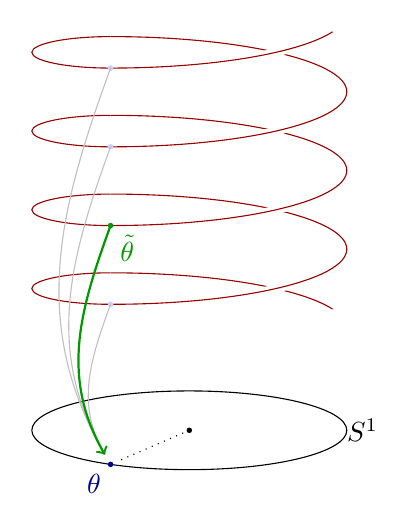
\begin{tikzpicture}[scale=1]
    \node[] (zero) at (0,0) {};
    \fill (zero) circle (1pt);
    \draw (0,-0.5) arc (270:-90:2 and 0.5);

    \node (theta) at ({cos(240) * 2},{sin(240) * 0.5}) {};
    % \node [below left of=theta,blue!40!white] {$\theta$};

    \draw[dotted] (0,0) -- (theta);
    \fill[blue!60!black] (theta) circle (1pt);


    \draw[red!60!black] (-1,2) arc (270:200:-3 and -0.7);
    \draw[line width=3pt,white] (-1,2) arc (270:90:1 and -0.2) arc (270:90:-3 and 0.7);
    \draw[red!60!black] (-1,2) arc (270:90:1 and -0.2) arc (270:90:-3 and 0.7);
    \fill[blue!20!white] (-1,1.6) circle (1pt);

    \draw[line width=3pt,white] (-1,3) arc (270:90:1 and -0.2) arc (270:90:-3 and 0.7);
    \draw[red!60!black] (-1,3) arc (270:90:1 and -0.2) arc (270:90:-3 and 0.7);
    \fill[green!60!black] (-1,2.6) circle (1pt);

    \draw[line width=3pt,white] (-1,4) arc (270:90:1 and -0.2) arc (270:90:-3 and 0.7);
    \draw[red!60!black] (-1,4) arc (270:90:1 and -0.2) arc (270:90:-3 and 0.7);
    \fill[blue!20!white] (-1,3.6) circle (1pt);

    \draw[line width=3pt,white] (-1,5) arc (270:90:1 and -0.2) arc (270:200:-3 and 0.7);
    \draw[red!60!black] (-1,5) arc (270:90:1 and -0.2) arc (270:200:-3 and 0.7);
    \fill[blue!20!white] (-1,4.6) circle (1pt);


    \draw[->,gray!50!white] (-1,1.6) to[out=250,in=120] (theta);
    \draw[->,gray!50!white] (-1,3.6) to[out=250,in=120] (theta);
    \draw[->,gray!50!white] (-1,4.6) to[out=250,in=120] (theta);
    \draw[->,green!60!black,thick] (-1,2.6) to[out=250,in=120] (theta);
    \node[below left,blue!60!black] at (theta) {$\theta$};
    \node[below right,green!60!black] at (-1,2.6) {$\tilde\theta$};

    \node[red!60!black] at (2.2,4.8) {$\R$};
    \node at (2.2,0) {$S^1$};
  \end{tikzpicture}
\end{center}

\textbf{$q$-sheet cover:}

\textbf{determination of a function:}

%%%%%%%%%%%%%%%%%%%%%%%%%%%%%%%%%%%%%%%%%%%%%%%%%%%%%%%%%%%%%%%%%%%%%%%%%%%%%%%
\subsubsection{Stokes directions / \dots}
\begin{comment}
  \cite[I.4]{Loday1994}
\end{comment}
We denote
\[
  \cQ_{[A^0]}:=\left\{q_1(t^{-1}),\dots,q_n(t^{-1})\right\}
\]
the set of the determining polynomials of $[A^0]$
\[
  \cQ_{[\End A^0]}:=\left\{\left(q_i-q_l\right)(t^{-1})
    \mid q_i \neq q_l \in\cQ_{[A^0]}
  \right\}
\]
the set of the determining polynomials of $[\End A^0]$ where\dots
\begin{defn}
  We call
  \begin{itemize}
    \item $a_{(j,l)}\in\C\backslash\{0\}$ the \emph{leading factor},
    \item $\frac{a_{(j,l)}}{t^k}=:q_{(j,l)}(t^{-1})$ the \emph{leading
      coefficient} and
    \item $k$ the \emph{degree} $\deg(q_j-q_l)$ of $(q_j-q_l)$ or a
      \emph{level} of $A^0$
  \end{itemize}
  of $q_j-q_l\in\cQ_{[\End A^0]}$ if
  \[
    q_j-q_l\in\left\{ \frac{a_{(j,l)}}{t^k}+h \mid h \in o(t^{-k})\right\} \,.
  \]
  \begin{rem}
    \begin{enumerate}
      \item In \cite{boalch} and \cite{thboalch} the $k$ is always an integer
        and is incremented by one. We will prefer the other definition, which
        is taken from \cite{Loday1994}, because \TODO
      \item In \cite[Def.4.3.6]{Loday2014} $a_{(j,l)}$ gets a negative sign to
        be consistend with calculations at $\infty$. Here this is not
        necessary, since we use then clockwise ordering.
    \end{enumerate}
  \end{rem}
  The degrees of the elements in $\cQ_{[\End A^0]}$ are the
  \emph{levels} of $A^0$.
  The set of all levels of $A^0$ will be denoted by
  \[
    \cK=\{k_1<\dots<k_r\} \subset \Q \,.
  \]
  \begin{rem}
    $A^0$ is unramified if and only if $\cK\subset\Z$. Since we only look at
    the unramified case, this will be always the case.
  \end{rem}
\end{defn}

On the elements of $\cQ(A^0)$ we define the following (partial) order
relations:
\begin{defn}
  \marginnote{\cite[Def.I.4.4]{Loday1994}}
  Let $\tilde\theta$ be a determination of $\theta$.
  We define the relations
  \begin{itemize}
    \item $\boldmath q_j \underset{\tilde\theta}{\prec} q_l$
      :\Leftrightarrow{} $\Re(a_{ij}e^{-ik\theta})<0$
    \\\Leftrightarrow{} $e^{(q_j-g_l)(t^{-1})}$ is
      flat\footnote{\TODO[define?]} at $0$ in a neighbourhood of the direction
      $\tilde\theta$.
    \item $\boldmath q_j \underset{\tilde\theta,\max}{\prec} q_l$
      :\Leftrightarrow{} $a_{ij}e^{-ik\tilde\theta}$ is a real negative number.
      \\\Leftrightarrow{} $e^{(q_j-g_l)(t^{-1})}$ is of maximal
      decay\footnote{\TODO[define?]} in the
      direction $\tilde\theta$.
      \begin{comment}
        \Leftrightarrow{} $q_{ij}(t^{-1})\in\R_{<0}$ along $\tilde\theta$.
      \end{comment}
  \end{itemize}
\end{defn}
\begin{rem}
  In the unramified case these relations do not depend on the determination
  $\tilde\theta$ of $\theta$. As a consequence we will only write
  $\underset{\theta}{\prec}$ and $\underset{\theta,\max}{\prec}$.
\end{rem}

\begin{defn}
  % \marginnote{See \cite[Def.I.4.5]{Loday1994}(for the ramified case)
  %   \cite[Def.3.2]{boalch}}
  \begin{enumerate}
    \item $\theta$ is an \emph{anti-Stokes direction} if there is at least one
      pair $(q_j,q_l)$ in $\cQ(A^0)$, which satisfies
      $q_j \underset{\theta,\max}{\prec} q_l$.
      \begin{itemize}
        \item Let $\A=\{\alpha_1,\dots,\alpha_{\nu}\}$ denote the set of all
          anti-Stokes directions in a clockwise ordering\footnote{In
          \cite{Loday1994} this ordering is chosen, since the calculations are
          then compatible with the calculations, which look at $\infty$ and take
          a counterclockwise ordering. \cite{boalch} and \cite{thboalch} use the
          inverse ordering, but look also at $0$.}. For a uniform notation
          later, define $\A$ to contain a single, arbitrary direction if $k=0$.
      \end{itemize}
    \item $\theta$ is an \emph{Stokes direction} when there is at least one
      pair $(q_j,q_l)$ in $\cQ(A^0)$, which satisfies neither
      $q_j\underset{\theta}{\prec} q_l$ nor $q_l\underset{\theta}{\prec} q_j$.
      \begin{itemize}
        \item Let $\S=\{\sigma_1<\cdots<\sigma_\mu\}$ be the set of Stokes
          directions.
      \end{itemize}
  \end{enumerate}
\end{defn}

\TODO

%%%%%%%%%%%%%%%%%%%%%%%%%%%%%%%%%%%%%%%%%%%%%%%%%%%%%%%%%%%%%%%%%%%%%%%%%%%%%%%
\subsubsection{Stokes group $\Sto_\theta(A^0)$}
\cite[Def.4.1]{hall2003lie} says the following about faithful
representations:
\begin{defn}
  \begin{comment}
    See:
    \begin{itemize}
      \item \cite[Def.4.1]{hall2003lie}
      \item \url{http://nlab.mathforge.org/nlab/show/faithful+representation}
    \end{itemize}
  \end{comment}
  Let $G$ bi a matrix Lie group. Then a \emph{(finite-dimensional complex)
  representation} of $G$ is a Lie group homomorphism
  \[
    \rho:G\to\Gl(V)
  \]
  where
  \begin{itemize}
    \item $V$ is a finite-dimensional complex vector space.
  \end{itemize}
  If $\rho$ is a one-to-one homomorphism, then the representation is called
  \emph{faithful}.
  \begin{comment}
    \textbf{Other criterion:}
    If the associated homomorphism $G\to\Aut(V)$ is injective, then the
    representation is \emph{faithful}.
  \end{comment}
  \begin{rem}
    If a representation $\rho$ is a faithful representation of a matrix Lie
    group $G$ then $\{\rho(A)\mid A\in G\}$ is a group of matrices that is
    isomorphic to the original group $G$. Thus, $\rho$ allows us to represent
    $G$ as a group of matrices.
  \end{rem}
\end{defn}
\begin{defn}
  Define the \emph{Stokes group}
  \[
    \Sto_\theta(A^0)=
    \left\{\phi_\theta\in\Lambda_\theta^{<0}(A^0)
      \mid \phi_\theta \text{ has maximal decay at } \theta
    \right\}
  \]
  and the group
  \[
    \SSto_d(A^0)= \left\{K\in G\mid K_{jl}=\delta_{jl} \text{ unless }
      q_j \underset{\theta,\max}{\prec} q_l \right\}
  \]
  which will arise as faithful representation of $\Sto_\theta(A^0)$.
  \begin{rem}
    For $\theta\notin\A$ the group $\Sto_\theta(A^0)$ is trivial, since no flat
    isotropy has maximal decay, but the identity.
  \end{rem}
\end{defn}
For every representation $\tilde\theta$ of $\theta$ there is an isomorphism
\[
  \rho_{\tilde\theta}:\Sto_\theta(A^0)\to\SSto_\theta(A^0)
\]
which maps a germ of $\Sto_\theta(A^0)$ to its faithful representation. This
process, in the case when $\theta\in\A$, is described as follows:
\begin{itemize}
  \item[] given
    \begin{itemize}
      \item a normal solution $X_0=t^\Lambda e^{Q(t^{-1})}$ and
      \item a determination $\tilde\theta$ of $\theta$.
    \end{itemize}
    Then denote by $X_{0,\tilde\theta}$ the function defined by $X_0$ with that
    determination of the argument near the direction $\theta$.
\end{itemize}
An element $\phi_\theta(t)\in\Sto_\theta(A^0)$ is thus a flat transformation
such that
\[
  \phi_\theta(t)X_{0,\tilde\theta}(t)
  =X_{0,\tilde\theta}(t)(1_n+C_{\tilde\theta})
\]
for a unique constant invertible matrix of the form $1_n+C_{\tilde\theta}$,
which we will call the \emph{representation of $\phi_\theta$}.
Some little reshaping results in the following equation
\[
  \phi_\theta(t)
  =t^\Lambda e^{Q(t^{-1})}(1_n+C_{\tilde\theta})e^{-Q(t^{-1})}t^{-\Lambda}
\]
and after decomposing \TODO[Fitting the structure of $Q$] $C_{\tilde\theta}$
into
\begin{align*}
  C_{\tilde\theta}&=\begin{pmatrix}
    c_{(1,1)} & c_{(1,2)} & \cdots &\\
    c_{(2,1} & \ddots\\
    \vdots \\
    & & & c_{(r,r)}
  \end{pmatrix}
\\&=
  \underset{C_{\tilde\theta}^{(1,1)}}{\underbrace{%
    \begin{pmatrix}
      c_{(1,1)} & 0 & \cdots &\\
      0\\
      \vdots&\\
      &
    \end{pmatrix}
  }}
  +
  \underset{C_{\tilde\theta}^{(1,2)}}{\underbrace{%
    \begin{pmatrix}
      0 & c_{(1,2)} & 0 & \cdots\\
      & 0 &\\
      &\vdots\\
      &
    \end{pmatrix}
  }}
  +\cdots+
  \underset{C_{\tilde\theta}^{(r,r)}}{\underbrace{%
    \begin{pmatrix}
      &\\
      & & & \vdots\\
      & & & 0\\
      & \cdots & 0 & c_{(r,r)}
    \end{pmatrix}
  }}
\\&=\sum_{(l,j)}C_{\tilde\theta}^{(l,j)}
\end{align*}
we get
\[
  \phi_\theta=
    t^\Lambda\left(
      1_n+\sum_{(l,j)}C_{\tilde\theta}^{(l,j)}e^{(q_l-q_j)(t^{-1})}
    \right)t^{-\Lambda} \,.
\]

\begin{paracol}{2}
\switchcolumn[0]\noindent
  Thus $\phi_\theta$ is flat in direction $\theta$ if and only if, as soon as
  $e^{(q_l-q_j)(t^{-1})}$ does not have maximal decay in direction
  $\tilde\theta$ the corresponding block $C_{\tilde\theta}^{(l,j)}$ is zero.
\switchcolumn[1]\noindent
  Thus, for $\phi_{\tilde\theta}$ to be flat in direction $\theta$, it is
  necessary and sufficient that if $e^{(q_l-q_j)(t^{-1})}$ does not have
  maximal decay in direction $\tilde\theta$ the corresponding
  block\footnote{\cite{Loday1994} talks about blocks, which correspond to the
  structure of $Q$.} $C_{\tilde\theta}^{(l,j)}$ vanishes.
\end{paracol}
In particular we get, that
\begin{itemize}
  \item for $j=l$ are the (diagonal) blocks $C_{\tilde\theta}^{(l,j)}$ are zero
    since $q_l-q_j=0$ and
  \item if $e^{q_j-q_l}$ has has maximal decay, then $e^{q_l-q_j}$. Thus if
    $C_{\tilde\theta}^{(l,j)}$ is not equal to zero, the block
    $C_{\tilde\theta}^{(j,l)}$ is necessarily zero.
\end{itemize}
This implies that the matrix $1_n+C_{\tilde\theta}$ is unipotent.
On the other hand, every constant unipotent Matrix, with zeros at the necessary
positions, characterizes a unique element of $\Sto_\theta(A^0)$.
Thus $\Sto_\alpha(A^0)$ is a unipotent Lie group.

\begin{lem}
  \marginnote{\cite[Def.I.4.12]{Loday1994}}
  A germ $\phi_\theta\in\Lambda_\theta(A^0)$ is a Stokes germ, i.e.\ an element
  in $\Sto_\theta(A^0)$ if and only if for some, hence all determination
  $\tilde\theta$, it has a representation $C_{\tilde\theta}$ of the form
  $ C_{\tilde\theta}=\sum_{(l,j)}C_{\tilde\theta}^{(l,j)}$.
\end{lem}
\begin{proof}
  See \cite[Def.I.4.12]{Loday1994}.
  \TODO
\end{proof}

\begin{comment}
  If we fix a normal solution $X_0=e^Le^{Q(1/x)}$
  \begin{lem}
    Each germ $\phi_\theta\in\Lambda_\theta(A^0)$ is representable, relative to
    $X_{0,\tilde\theta}$, by a unique matrix
    \[
      C_{X_{0,\tilde\theta}}=
        1+\sum_{(j,l)\mid q_j \underset{\theta}{\prec} q_l} c_{(j,l)}E_{(j,l)}
    \]
    such that $\phi_\theta(x)
    =X_{0,\tilde\theta}(x)C_{X_{0,\tilde\theta}}X_{0,\tilde\theta}(x)^{-1}$ near
    $\theta$.

    \TODO

    \marginnote{\cite[Con.I.4.8]{Loday1994}}
    Thus the sheaf $\Lambda(A^0)$ is a sheaf of non-Abelian unipotent groups.
  \end{lem}
\end{comment}

\begin{notations}
  \marginnote{\cite[Not.I.4.15]{Loday1994}}
  For $k\in\cK$ and $\theta\in\A$ we set:
  \begin{itemize}
    \item $\Lambda^{k}(A^0):=$ the subsheaf of $\Lambda(A^0)$ of all germs,
      which are generated by $k$-germs;
    \item $\Lambda^{\leq k}(A^0)$ (resp. $\Lambda^{<k}(A^0)$) as the subsheaf
      of $\Lambda(A^0)$ generated by $k'$-germs for all $k'\leq k$ (resp.
      $k'<k$);
    \item $\Sto_\theta^k(A^0):=\Sto_\theta(A^0)\cap\Lambda_\theta^{k}(A^0)$;
    \item $\Sto_\theta^{\leq k}(A^0):=\Sto_\theta(A^0)\cap\Lambda_\theta^{\leq k}(A^0)$;
    \item $\Sto_\theta^{<k}(A^0):=\Sto_\theta(A^0)\cap\Lambda_\theta^{<k}(A^0)$;
    \item $\A^k:=\left\{\theta\in\A\mid\Sto_\theta^k(A^0\neq\{1\})\right\}$ the
      set of anti-Stokes directions \emph{bearing the level $k$};
    \item $\A^{\leq k}:=\underset{k'\leq k}\bigcup\A^{k'}$ (resp.
      $\A^{<k}:=\underset{k'<k}\bigcup\A^{k'}$);
    \item $\cK_\theta:=\left\{k\in\cK\mid\Sto_\theta^k(A^0)\neq\{1\}\right\}$
      the set of levels \emph{beared by $\theta\in\A$}.
  \end{itemize}
\end{notations}
\begin{rem}
  We clearly have the canonical inclusions
  \begin{itemize}
    \item $\cA^k\hookrightarrow \cA^{\leq k}$ and
    \item $\cA^{<k}\hookrightarrow \cA^{\leq k}$.
  \end{itemize}
\end{rem}

%%%%%%%%%%%%%%%%%%%%%%%%%%%%%%%%%%%%%%%%%%%%%%%%%%%%%%%%%%%%%%%%%%%%%%%%%%%%%%%
\subsubsection{Filtration of \TODO{} by levels}
\marginnote{See \cite[I.5]{Loday1994} (See [LR91])}
\begin{prop}
  \marginnote{\cite[Prop.I.5.1]{Loday1994}}
  For any level $k\in\cK$ one has
  \begin{enumerate}
    \item $\Lambda^{k}(A^0)$, $\Lambda^{\leq k}(A^0)$ and $\Lambda^{<k}(A^0)$
      are sheaves of subgroups of $\Lambda(A^0)$;
    \item $\Lambda^k(A^0)$ is normal in $\Lambda^{\leq k}(A^0)$;
    \item the exact sequence of sheaves
      \[
        1\to\Lambda^k(A^0)
        \overset{i}\to\Lambda^{\leq k}(A^0)
        \overset{p}\to\Lambda^{<k}(A^0)
        \to 1
      \]
      splits.
  \end{enumerate}
\end{prop}
\begin{proof}
  \begin{enumerate}
    \item \TODO{}
    \item \TODO{}
    \item This is clear, since we have the canonical inclusion
      $\Lambda^{<k}(A^0)\hookrightarrow\Lambda^{\leq k}(A^0)$.
  \end{enumerate}
\end{proof}
\begin{comment}
  \begin{cor}
    \cite[Cor.I.5.2]{Loday1994} says:\\
  \end{cor}
  \begin{prop}
    \cite[Prop.I.5.3]{Loday1994} says:\\
  \end{prop}
  \begin{proof}
    \TODO{}
  \end{proof}
  \begin{cor}
    \cite[Cor.I.5.4]{Loday1994} says:\\
    \TODO
    \[
      \Lambda(A^0)\cong\underset{k\in\cK_\theta}\ltimes\Lambda^k(A^0)
    \]
    taken in arbitrary order.
  \end{cor}
  \begin{proof}
    \TODO{}
  \end{proof}
  \begin{prop}
    \cite[Prop.I.5.5]{Loday1994} says:\\
    The results can be restricted to the Stokes groups. Thus, for
    $\theta\in\A$, one has
    \[
      \Sto_\theta(A^0)\cong\underset{k\in\cK_\theta}\ltimes\Sto_\theta^k(A^0)
    \]
    the semi-direct product being taken in an arbitrary order.
  \end{prop}
  \begin{proof}
    \TODO{}
  \end{proof}
\end{comment}

%%%%%%%%%%%%%%%%%%%%%%%%%%%%%%%%%%%%%%%%%%%%%%%%%%%%%%%%%%%%%%%%%%%%%%%%%%%%%%%
\subsection{The theorem}
\marginnote{\cite[868]{Loday1994}}
Let $\{\theta_j\mid j\in J\}\subset S^1$ be a finite set and
$\dot\phi=(\dot\phi_{\theta_j})_{j\in J}\in\prod_{j\in J}\Lambda_{\theta_j}(A^0)$
be a finite family of germs.
In the following way, one can associate a cohomology class to any $\dot\phi$:
let $\dot\phi_j$ be the function representing the germ $\dot\phi_{\theta_j}$ on
its maximal arc of definition $\Omega_j$ around $\theta_j$.
When a cyclic covering $\cU=\{U_j;j\in J\}$ satisfies
$\dot U_j\subset \Omega_j$ for all $j\in J$ one can define the $1$-cocycle
$(\dot\phi_{j|\dot U_j})_{j\in J}$ on $\cU$.
To a differente $\cU$ this construction yields a cohomologous
$1$-cocycle\TODO[Proof], thus the resulting map, in the case
$\{\theta_j\mid j\in J\}=\A$,
\[
  h:\prod_{\alpha\in\A}\Sto_\alpha(A^0)\to
  H^1(A^1;\Lambda(A^0))=\St(A^0)
\]
is welldefined.
\begin{tthm}
  \label{thm:mainThm2}
  The map
  \[
    h:\prod_{\alpha\in\A}\Sto_\alpha(A^0)\to\St(A^0)
  \]
  is a bijection and natural.
  \begin{rem}
    \marginnote{\cite[869]{Loday1994}}
    Natural means that $h$ commutes to isomorphisms and constructions over
    systems or connections they represent.
    \begin{comment}
      See \cite{Loday1994} Section III.3.3
    \end{comment}
  \end{rem}
\end{tthm}
From theorem~\ref{thm:mainThm2} and \TODO{} we get the following corollary.
\begin{cor}
  \[
    \St(A^0) \cong \prod_{\alpha\in\A}\SSto_\alpha(A^0)
  \]
  and thus has complex dimension \TODO{}
\end{cor}
%%%%%%%%%%%%%%%%%%%%%%%%%%%%%%%%%%%%%%%%%%%%%%%%%%%%%%%%%%%%%%%%%%%%%%%%%%%%%%%
\subsection{Proof}
We will only look at the unramified case, for which we refer to
\cite[Sec.II.3]{Loday1994}.
The proof in the ramified case can be found in \cite[Sec.II.4]{Loday1994}.

%%%%%%%%%%%%%%%%%%%%%%%%%%%%%%%%%%%%%%%%%%%%%%%%%%%%%%%%%%%%%%%%%%%%%%%%%%%%%%%
\subsubsection{The case of a unique level}
\begin{comment}
  \cite[II.3.2]{Loday1994}
\end{comment}
First we will look at the case of a unique level. This means that
\begin{itemize}
  \item $\Lambda(A^0)$ has only one level $k$, thus
    \begin{itemize}
      \item $\Lambda(A^0)=\Lambda^k(A^0)$ and
      \item $\Sto_\theta(A^0)=\Sto_\theta^k(A^0)$.
    \end{itemize}
  \item Or we restrict to a given level $k\in\cK$.
\end{itemize}
\begin{lem}
  Let $k\in\cK$.
  The canonical injective map
  \[
    i^k:\underset{\theta\in\A}\prod\Sto_\theta^k(A^0) \to
    \Gamma(\dot\cU^k;\Lambda^k(A^0))
  \]
  and the canonical surjective map
  \[
    s^k:\Gamma(\dot\cU^k;\Lambda^k(A^0))\to H^1(S^1;\Lambda^k(A^0))
  \]
  are bijective and thus
  \[
    \underset{\theta\in\A}\prod\Sto_\theta^k(A^0)
    \underset{\sim}{\overset{i^k}{\longrightarrow}}
    \Gamma(\dot\cU^k;\Lambda^k(A^0))
    \underset{\sim}{\overset{s^k}{\longrightarrow}}
    H^1(S^1;\Lambda^k(A^0))
  \]
  is a bijection.
\end{lem}
\begin{proof}
  \begin{enumerate}
    \item The map $i^k$ is the canonical extension of germs to their natural
      arc of definition and thus a group isomorphism.
    \item The map $s^k$ is the quotient map. \TODO{}
  \end{enumerate}
\end{proof}

%%%%%%%%%%%%%%%%%%%%%%%%%%%%%%%%%%%%%%%%%%%%%%%%%%%%%%%%%%%%%%%%%%%%%%%%%%%%%%%
\subsubsection{The case of a several level}
\begin{comment}
  \cite[II.3.3]{Loday1994}
\end{comment}
\begin{defn}
  We want to define a \emph{product map of cocycles} $\mathfrak{S}^{\leq k}$.
  This map will be composed from the following injective maps:
  \begin{enumerate}
    \item The first map is defined as
      \begin{align*}
        \sigma^k:\Gamma(\dot\cU^k;\Lambda^k(A^0))
        &\to \Gamma(\dot\cU^{\leq k};\Lambda^{\leq k}(A^0))
      \\\dot f=(\dot f_\theta)_{\theta\in\A^k}
        &\mapsto (\dot G_\theta)_{\theta\in\A^{\leq k}}
      \end{align*}
      where
      \begin{itemize}
        \item $\dot G_\theta=\begin{cases}
            \dot f_\alpha \text{~restricted to } \dot U_\theta^{\leq k}
            \text{~and seen as being in } \Lambda^{\leq k}(A^0)
            & \text{~when } \theta\in\A^k
          \\1 \text{~(the identity) }
            & \text{~when } \theta\notin\A^k
          \end{cases}$
      \end{itemize}
    \item and the second map
      \begin{align*}
        \sigma^{<k}:\Gamma(\dot\cU^{<k};\Lambda^{<k}(A^0))
        &\to \Gamma(\dot\cU^{\leq k};\Lambda^{\leq k}(A^0))
      \\\dot f=(\dot f_\theta)_{\theta\in\A^{<k}}
        &\mapsto (\dot F_\theta)_{\theta\in\A^{\leq k}}
      \end{align*}
      is defined in a similar way as
      \begin{itemize}
        \item $\dot G_\theta=\begin{cases}
            \dot f_\alpha \text{~restricted to } \dot U_\theta^{\leq k}
            \text{~and seen as being in } \Lambda^{\leq k}(A^0)
            & \text{~when } \theta\in\A^{<k}
          \\1 \text{~(the identity) }
            & \text{~when } \theta\notin\A^{<k}
          \end{cases}$
      \end{itemize}
  \end{enumerate}
  Thus we can define
  \begin{align*}
    \mathfrak{S}^{\leq k}:
    \Gamma(\dot\cU^{<k};\Lambda^{<k}(A^0))
    \times
    \Gamma(\dot\cU^{k};\Lambda^{k}(A^0))
    &\to
    \Gamma(\dot\cU^{\leq k};\Lambda^{\leq k}(A^0))
  \\(\dot f, \dot g)
    &\mapsto
    (\dot F_\theta\dot G_\theta)_{\theta\in\A^{\leq k}}
  \end{align*}
  where $(\dot F_\theta)_{\theta\in\A^{\leq k}}=\sigma^{<k}(\dot f)$ and
  $(\dot G_\theta)_{\theta\in\A^{\leq k}}=\sigma^{<k}(\dot g)$ as defined
  above.
  \begin{rem}
    This map is injective, since injectivity for germs implies injectivity for
    sections.
  \end{rem}
\end{defn}

\begin{lem}
  \marginnote{\cite[Lem.II.3.3]{Loday1994}}
  Let $k\in\cK$.
  \begin{enumerate}
    \item If the cocycles $\mathfrak{S}^{\leq k}(\dot f,\dot g)$ and
      $\mathfrak{S}^{\leq k}(\dot f',\dot g')$ are cohomologous in
      $\Gamma(\dot\cU^{\leq k};\Lambda^{\leq k}(A^0))$
      then $\dot f$ and $\dot f'$ are cohomologous in
      $\Gamma(\dot\cU^{<k};\Lambda^{<k}(A^0))$.
    \item Any cocycle in $\Gamma(\dot\cU^{\leq k},\Lambda^{\leq k}(A^0))$ is
      cohomologous to a cocycle in the range of $\mathfrak{S}^{\leq k}$.
  \end{enumerate}
\end{lem}
\begin{proof}
  \begin{comment}
    See \cite[Lem.II.3.3]{Loday1994}.
  \end{comment}
  \begin{enumerate}
    \item
      Denote by $\theta^+$ the nearest anti-Stokes direction in $\A^{\leq k}$
      on the right\footnote{In clockwise direction.} of $\theta$.
      \TODO{}
    \item \TODO{}
  \end{enumerate}
  \TODO{}
\end{proof}
\begin{defn}
  Define the injective map
  \begin{align}
    \tau^k:\Gamma(\dot\cU^k;\Lambda^k(A^0)) &\to \Gamma(\dot\cU;\Lambda(A^0))
  \\\dot f=(\dot f_\theta)_{\theta\in\A^k} &\mapsto
    (\dot F_\theta)_{\theta\in\A}
  \end{align}
  where
  \[
    \dot F_\theta=\begin{cases}
      \dot f_\alpha \text{~restricted to } \dot U_\theta
      \text{~and seen as being in } \Lambda(A^0)
      & \text{~when } \theta\in\A^k
    \\1 \text{~(the identity) }
      & \text{~when } \theta\notin\A^k
    \end{cases} \,.
  \]
  \marginnote{\cite[Prop.II.3.4]{Loday1994}}
  The \emph{product map of single-leveled cocycles} is then defined as
  \begin{align*}
    \tau:\prod_{k\in\cK}\Gamma(\dot \cU^k;\Lambda^k(A^0))
    &\to
    \Gamma(\dot\cU;\Lambda(A^0))
  \\(\dot f^k)_{k\in\cK}i
    &\mapsto
    \prod_{k\in\cK}\tau^k(\dot f^k)
  \end{align*}
  following an ascending order of levels.
  \begin{rem}
    \begin{enumerate}
      \item This map, again, is injective.
        \TODO[proof?]
      \item It can be extended to an arbitrary order of levels.
    \end{enumerate}
  \end{rem}
\end{defn}
\begin{cor}
  The product map of single-leveled cocycles induces on the cohomology
  a bijective and natural map
  \[
    \cT:
    \underset{\underset{k\in\cK}\prod H^1(S^1;\Lambda^k(A^0))}{%
      \underset{\text{\rotatebox[origin=c]{-90}{$\cong$}}}{%
        \prod_{k\in\cK}\Gamma(\dot\cU^k;\Lambda^k(A^0))}}
    \longrightarrow
    \underset{H^1(S^1;\Lambda(A^0))}{%
      \underset{\text{\rotatebox[origin=c]{-90}{$\cong$}}}{%
        H^1(\cU;\Lambda(A^0))}}\,.
  \]
\end{cor}
\begin{proof}
  \TODO{}
\end{proof}
\subsubsection{Composing functions to obtain $h$}
Thus, we are now able to create the function $h$ from
theoreme~\ref{thm:mainThm2} by composition of bijective maps.
\begin{proof}[Proof of theoreme~\ref{thm:mainThm2}]
  Let us denote the composition
  \[
    \prod_{\theta\in\cA}\Sto_\theta(A^0)
    \overset{\prod_{\theta\in\A}i_\theta}{\xrightarrow{\hspace*{1.2cm}}}
    \prod_{\theta\in\cA}\prod_{k\in\cK}\Sto_\theta^k(A^0)
    \equiv
    \prod_{k\in\cK}\prod_{\theta\in\cA}\Sto_\theta^k(A^0)
    \overset{\prod_{k\in\cK}i^k}{\xrightarrow{\hspace*{1.2cm}}}
    \prod_{k\in\cK}\Gamma(\dot\cU^k;\Lambda^k(A^0))
    \,,
  \]
  where
  \begin{itemize}
    \item $i_\theta:\Sto_\theta(A^0)\to\prod_{k\in\cK}\Sto_\theta^k(A^0)$ gives
      \TODO{} and
    \item $i^k:\prod_{\theta\in\cA}\Sto_\theta^k(A^0)
      \to\Gamma(\dot\cU^k;\Lambda^k(A^0))$ is the canonical map,
  \end{itemize}
  by $\mathfrak{T}$. Thus we obtain the bijection
  \[
    \cT\circ\mathfrak{T}:
    \prod_{\theta\in\cA}\Sto_\theta(A^0)
    \to
    H^1(\cU;\Lambda(A^0))
  \]
  as the map $h$.
  \TODO[naturality (is obvious?)]
\end{proof}
